
%(BEGIN_QUESTION)
% Copyright 2010, Tony R. Kuphaldt, released under the Creative Commons Attribution License (v 1.0)
% This means you may do almost anything with this work of mine, so long as you give me proper credit

Suppose a technician needs to test a pair of wires in a newly-installed multi-pair cable for open and short faults.  The cable ends are terminated at terminal blocks too far away to permit a multimeter's test leads to stretch from one end to the other:

$$\includegraphics[width=15.5cm]{i02263x01.eps}$$

Devise a series of measurements that a technician could take using a multimeter located at one end of the cable.  Be sure to specify which setting the multimeter should be configured for, and which terminals the test leads should touch.  Also, be sure to specify what range of measurements would indicate ``good'' versus ``bad'' for each test:

\begin{itemize}
\item{} Pair ``A'' wires shorted together in cable
\vskip 10pt
\item{} Either conductor of Pair ``A'' being broken (open)
\vskip 10pt
\item{} Either conductor of Pair ``A'' shorted to cable shield
\end{itemize}

\vfil 

\underbar{file i02263}
\eject
%(END_QUESTION)





%(BEGIN_ANSWER)

This is a graded question -- no answers or hints given!

%(END_ANSWER)





%(BEGIN_NOTES)

Fundamental concepts to bear in mind here are that ``shorted'' faults exhibit low resistance, while ``open'' faults exhibit extremely high (nearly infinite) resistance.  If we need to test a cable for the presence of any shorted faults, we must connect an ohmmeter to the cable in such a way that the presence of such a short will be registered on the meter: i.e. between the potentially shorted points, looking for an abnormally low resistance.  If we need to test a cable for the presence of any open faults, we must connect the ohmmeter in such a way that the presence of an open will be registered: i.e. between points which ought to be connected, looking for an abnormally high resistance.

\vskip 10pt

The most challenging of these three tests is the end-to-end continuity test of pair A, requiring us to first ``jumper'' the far end of this wire pair to establish continuity before we attempt to measure the resistance of that wire loop.

\vskip 10pt

\begin{itemize}
\item{} Pair A wires shorted together in cable: {\it measure resistance between terminals 1 and 2.  High resistance is good, while low resistance indicates a short.}
\vskip 10pt
\item{} Either conductor of Pair A being broken (open): {\it short terminals 1 and 2 together at one end of the cable, then measure resistance between terminals 1 and 2 at the other end of the cable.  Low resistance is good, while high resistance indicates an open.}
\vskip 10pt
\item{} Either conductor of Pair A shorted to cable shield: {\it measure resistance between terminals 1 and 7, then between 2 and 7.  High resistance in either case is good, while low resistance in either case indicates a short.}
\end{itemize}

%INDEX% Electronics review: continuity-checking a multi-pair cable

%(END_NOTES)

